%
% chapter.tex -- Kapitel 5: Der Satz von Gauss
%
% (c) 2024 Prof Dr Andreas Müller
%
\chapter{Der Satz von Gauss
\label{chapter:gauss}}
\kopflinks{Der Satz von Gauss}

\noindent
In den vorangegangenen Kapiteln wurden $p$-Formen betrachtet mit
$p\in\{0,1,2\}$, es wurde ein Ableitungsoperator $d$ definiert
und die Integration über $p$-dimensionale Untermannigfaltigkeiten $M$
und über den Rand $\partial M$.
Die Sätze von Green und Stokes haben gezeigt, dass den Zusammenhang
\begin{equation}
\int_M d\omega = \int_{\partial M} \omega
\label{buch:gauss:eqn:stokes}
\end{equation}
zwischen dem Integral der Ableitung einer $p-1$-Form über eine
$p$-dimensionale Mannigfaltigkeit und dem Integral der ursprünglichen
Form über den $p-1$-dimensionalen Rand gibt.
Der nächste Schritt ist daher, einen Zusammenhang zwischen dem Volumenintegral
einer 3-Form über einen Körper und einem Oberflächenintegral
einer 2-Form über die geschlossen Fläche, die den Rand des Körpers bildet,
herstellt.
Dieser Zusammenhang ist bekannt als der Satz von Gauss und der
Differentialoperator ist die Divergenz.

Die Divergenz der Strömung eines Fluids beschreibt, in welchem Ausmass
in einem gegebenen Raumvolumen neues Fluid entsteht.
Eine $n-1$-Form beschreibt dann den Fluss des Fluids durch die Oberfläche.
Die Erhaltung der Menge des Fluids muss sich also als Gleichung
von Integralen wie in \eqref{buch:gauss:eqn:stokes} oder als
Differentialgleichung mit der Divergenz schreiben lassen.
Solche Feldgleichungen gehören zu den wichtigsten und in fast allen
Anwendungen der Feldtheorie auftretenden Gleichungen.
Sie werden in Abschnitt~\ref{buch:gauss:section:erhaltungssatz}
genauer untersucht.

%
% Der Satz von Gauss in Dimension n=3
%
\section{Der Satz von Gauss in Dimension $n=3$
\label{buch:gauss:section:dimension3}}
\kopfrechts{Der Satz von Gauss in Dimension $n=3$}
Die Sätze von Green und Stokes haben gezeigt, wie sich das Verhalten
einer Ableitung im Inneren eines zweidimensionalen Gebietes oder
einer im Raum eingetteten Fläche aus den Werten auf dem Rand erschliessen
lässt.
Er verallgemeinert den Hauptsatz der Infinitesimalrechnung, der dieselbe
Art von Aussage für eindimensionale Gebiete oder In den Raum eingebettete
Kurven macht.
Es gibt aber keinen Grund, bei den Dimensionen 1 und 2 stehen zu bleiben.
In diesem Abschnitt wird der Fall $n-1=2$ und $n=3$ genauer untersucht,
der traditionell als der Satz von Gauss bekannt ist.
Im nächsten Abschnitt wird dies dann auf beliebige Dimension verallgemeinert.

Die Vorgehensweise ist völlig analog zum zweidimensionalen Fall.
Die Argumente werden daher teilweise nicht im gleichen Detail
wie in Kapitel~\ref{chapter:green} präsentiert.

%
% Integration auf dreidimensioinalen Mannigfaltigkeiten
%
\subsection{Integration auf dreidimensionalen Mannigfaltigkeiten}
Zunächst muss die Integration von zwei auf drei Dimensionen erweitert
werden.
Dabei tauchen als natürliche Konstrukte die Begriff von 3-Vektor und
3-Form auf.

\subsubsection{Dreifache Integrale}
Sei $f\colon U\to\mathbb{R}:(x,y,z)\mapsto f(x,y,z)$ eine
stetige Funktion, die in einer offenen Teilmenge $U\subset\mathbb{R}^3$
definiert ist.
Wir betrachten ein Gebiet $V\subset U$, welches
durch die Ungleichungen
\[
x_-\le x \le x_+,
\qquad
y_-(x)\le y\le y_+(x)
\qquad\text{und}\qquad
z_-(x,y)\le z\le z_+(x,y)
\]
beschrieben werden kann, wobei die Funktionen $y_{\pm}$ und $z_{\pm}$
ebenfalls stetig sein sollen.

Das (dreifache) Integral der Funktion $f$ über die Menge $V$ ist dann durch 
das iterierte Integral
\begin{align}
\underset{V}{\int\!\!\!\int\!\!\!\int}
f(x,y,z)\,dx\,dy\,z
&=
\int_{x_-}^{x_+}
\int_{y_-(x)}^{y_+(x)}
\int_{z_-(x,y)}^{z_+(x,y)}
f(x,y,z)
\,dz
\,dy
\,dx
\label{buch:gauss:3d:eqn:integral}
\end{align}
gegeben.
Der Satz von Fubini besagt, dass eine alternative Beschreibung des
Gebietes zum Beispiel durch Ungleichungen der Form
\[
y_-\le y \le y_+,
\qquad
z_-(y)\le z\le z_+(y)
\qquad\text{und}\qquad
x_-(y,z)\le x\le x_+(y,z)
\]
auf den gleichen Wert
\begin{align*}
\underset{V}{\int\!\!\!\int\!\!\!\int}
f(x,y,z)\,dx\,dy\,z
&=
\int_{y_-}^{y_+}
\int_{z_-(y)}^{z_+(y)}
\int_{x_-(y,z)}^{x_+(y,z)}
f(x,y,z)
\,dx
\,dz
\,dy
\end{align*}
führt.

%
% Volumenelement
%
\subsubsection{Volumenelement}
Der Ausdruck $dx\,dy\,dz$ in \eqref{buch:gauss:3d:eqn:integral}
wird auch als das Volumenelement in kartesischen Koordinaten bezeichnet.
Man stellt sich das Gebiet $V$ zusammengesetzt aus kleinen Quadern
an der Stelle $(x_i,y_i,z_i)$, $i=1,\dots,N$,
mit Seitenlängen $\Delta x$, $\Delta y$ und $\Delta z$, die ein
Volumen $\Delta x\,\Delta y\,\Delta z$ haben.
Dann bildet man riemannsche Summen
\[
I_N
=
\sum_{i=1}^N
f(x_i,y_i,z_i)\,\Delta x\,\Delta y\,\Delta z
\]
und lässt dann $N\to\infty$ gehen, wobei gleichzeitig die Kantenlängen
der Quader gegen Null gehen sollen.
Der Grenzwert
\[
\lim_{N\to\infty} I_N
=:
\underset{V}{\int\!\!\!\int\!\!\!\int}
f(x,y,z)\,dx\,dy\,z
\]
heisst, sofern er existiert, das Riemannsche Integral der Funktion $f$
über $V$.

%
% Koordinatenwechsel
%
\subsubsection{Koordinatenwechsel}
Wir betrachten jetzt die Wirkung eines Koordinatenwechsels.
Um die Notation etwas leichter nachvollziehbar zu gestalten, schreiben
wir die Koordinaten wieder in Indexnotation.
Die glatten Funktionen
\begin{equation}
y^i
=
y^i(x^1,x^2,x^3),\quad i\in\{1,2,3\}
\label{buch:gauss:3d:eqn:koordinatenabbildung}
\end{equation}
beschreiben den Wechsel der Koordinaten.

Das Volumenelement in den $x$-Koordinaten entsteht aus der Vorstellung
von kleinen Quadern mit Seitenkanten der Länge
$\Delta x^1$, 
$\Delta x^2$ und
$\Delta x^3$.
Die Kanten können durch die Standardbasisvektoren $\vec{e}_i$ als
$\vec{e}_1\Delta x^1$, $\vec{e}_2\Delta x^2$ und $\vec{e}_e\Delta x^3$
dargestellt werden.

Die Koordinatenabbildung~\eqref{buch:gauss:3d:eqn:koordinatenabbildung}
deformiert den Quader zu Körper mit gekrümmten Seitenkanten.
Für genügend kleine $\Delta x^i$ kann er approximiert werden durch
ein Parallelepiped mit den Seitenkante
\[
Dy\cdot(\vec{e}_i\Delta x^i)
=
\Delta x^i
\frac{\partial(y^1,y^2,y^3)}{\partial(x^1,x^2,x^3)}
\vec{e}_i
=
\Delta x^i
\renewcommand{\arraystretch}{2.0}
\begin{pmatrix}
\displaystyle\frac{\partial y^1}{\partial x^1}&
\displaystyle\frac{\partial y^1}{\partial x^2}&
\displaystyle\frac{\partial y^1}{\partial x^3}\\
\displaystyle\frac{\partial y^2}{\partial x^1}&
\displaystyle\frac{\partial y^2}{\partial x^2}&
\displaystyle\frac{\partial y^2}{\partial x^3}\\
\displaystyle\frac{\partial y^3}{\partial x^1}&
\displaystyle\frac{\partial y^3}{\partial x^2}&
\displaystyle\frac{\partial y^3}{\partial x^3}
\end{pmatrix}
\vec{e}_i
=
\Delta x^i
\begin{pmatrix}
\displaystyle\frac{\partial y^1}{\partial x^i}\\
\displaystyle\frac{\partial y^2}{\partial x^i}\\
\displaystyle\frac{\partial y^3}{\partial x^i}\\
\end{pmatrix}
\]
Die Funktionalmatrix $Dy$ bildet die Kantenvektoren ab.

Das Volumen des von den Vektoren $Dy\cdot\vec{e}_i$ aufgespannten
Parallelepipeds wird durch die Determinaten $\det Dy$ der
Abbildungsmatrix gegeben. 
Ist die Funktion $f$ in $y$-Koordinaten als $f(y^1,y^2,y^3)$ gegeben 
ist das Integral von $f$ daher 
\begin{align*}
\int\!\!\!\int\!\!\!\int
\tilde{f}(y_1,y_2,y_3)
\,dy^1
\,dy^2
\,dy^3
&=
\int\!\!\!\int\!\!\!\int
f(x^1,x^2,x^3)
\left|
\frac{\partial (y^1,y^2,y^3)}{\partial(x^1,x^2,x^3)}
\right|
\,dx^1
\,dx^2
\,dx^3.
\\
&=
\int\!\!\!\int\!\!\!\int
f(x^1,x^2,x^3)
\det Dy(x^1,x^2,x^3)
\,dx^1
\,dx^2
\,dx^3.
\end{align*}
Das Integral einer Funktion ist also nicht koordinatenunabhängig:

%
% 3-Vektoren
%
\subsubsection{3-Vektoren}
In Abschnitt~\ref{buch:green:section:integral} wurde dargestellt, wie
das Integral einer 2-Form definiert werden kann.
Dabei wurde ausführlich erklärt, wie eine 2-Form die richtigen
Transformationseigenschaften hat, damit das Integral der 2-Form
eine koordinatenaunabhängige Grösse wird.
Wir übertragen daher die Definition von 2-Fektoren und 2-Formen
auf den dreidimensionalen Fall.

Ein 3-Vektor ist eine Linearkombination von Tensoren dritter Stufe
Die drei Faktoren müssen vollständig antisymmetrisch sein.
Jede Vertauschung muss das Vorzeichen kehren.
Dies führt auf die komplizierte Summe
\begin{align}
\vec{e}_i
\wedge
\vec{e}_k
\wedge
\vec{e}_l
&=
\phantom{+}
\vec{e}_i\otimes\vec{e}_k\otimes\vec{e}_l
+
\vec{e}_k\otimes\vec{e}_l\otimes\vec{e}_i
+
\vec{e}_l\otimes\vec{e}_i\otimes\vec{e}_k
\\
&\phantom{=}
-
\vec{e}_i\otimes\vec{e}_l\otimes\vec{e}_k
-
\vec{e}_l\otimes\vec{e}_k\otimes\vec{e}_i
-
\vec{e}_k\otimes\vec{e}_i\otimes\vec{e}_l.
\label{buch:gauss:3d:eqn:3vektor}
\end{align}
Um solche Ausdrücke einfacher schreiben zu können führen wir das
Levi-Cività-Symbol ein.
Dazu brauchen wir zunächst den Begriff der geraden bzw.~ungeraden
Permutation.

\begin{definition}[Gerade und ungerade Permutation]
Eine Permutation $i_1,\dots,i_n$ der Zahlen $1,\dots,n$ heisst {\em gerade},
wenn sie durch eine gerade Anzahl Vertauschungen von aus $1,\dots,n$
entsteht.
Sie heisst {\em ungerade}, wenn eine ungerade Anzahl Vertauschungen
nötig ist
\index{gerade Permutation}%
\index{ungerade Permutation}%
\end{definition}

Für $n=2$ sind $(1,2)$ und $(2,1)$ die einzigen Permutationen,
die erste ist gerade, die zweite ungerade.
Für $n=3$ gibt es insgesamt 6 Permutationen, nämlich
\[
\begin{aligned}
&\text{gerade:}  &&(1,2,3),\;(2,3,1),\;(3,1,2)\\
&\text{ungerade:}&&(1,3,2),\;(3,2,1),\;(2,1,3).
\end{aligned}
\]
Für die Formel \eqref{buch:gauss:3d:eqn:3vektor} ist vor allem
das Vorzeichen der einzelnen Terme wichtig.
Das Levi-Cività-Symbol definiert dieses.

\begin{definition}[Levi-Cività-Symbol]
Das Levi-Cività-Symbol $n$-ter Stufe ist definiert durch
\[
\varepsilon_{i_1\dots i_n}
=
\begin{cases}
\phantom{-}1&\qquad\text{$i_1,\dots,i_n$ ist eine gerade Permutation}\\
         - 1&\qquad\text{$i_1,\dots,i_n$ ist eine ungerade Permutation}\\
\phantom{-}0&\qquad\text{sonst}
\end{cases}
\]
\end{definition}

Mit dem Levi-Cività-Symbol kann man 
\eqref{buch:gauss:3d:eqn:3vektor}
als
\[
\vec{e}_1
\wedge
\vec{e}_2
\wedge
\vec{e}_3
=
\sum_{i_1,\dots,i_n=1}^n
\varepsilon_{i_1 i_2 i_3}
\vec{e}_{i_1}
\otimes
\vec{e}_{i_2}
\otimes
\vec{e}_{i_3}
\]
schreiben.
Für Tensorfelder auf einer Mannigfaltigkeit kann auch die Schreibweise
\[
\frac{\partial}{\partial x^1}
\wedge
\frac{\partial}{\partial x^1}
\wedge
\frac{\partial}{\partial x^1}
=
\sum_{i_1,\dots,i_3=1}^3
\varepsilon_{i_1 i_2 i_3}
\frac{\partial}{\partial x^{i_1}}
\otimes
\frac{\partial}{\partial x^{i_2}}
\otimes
\frac{\partial}{\partial x^{i_3}}
\]
verwendet werden.
So wie es in zwei Dimensionen der Raum der 2-Vektoren eindimensional
war, ist in drei Dimensionen der Raum der 3-Vektoren eindimensional
und $\vec{e}_1\wedge\vec{e}_2\wedge\vec{e}_3$ kann als Basisvektor
betrachtet werden.

%
% 3-Formen
%
\subsubsection{3-Formen}
Dual zum Konzept des 3-Vektors können wir auch die 3-Formen
\[
\omega(x)
=
f(x)
dx^1 \wedge dx^2 \wedge dx^3
\]
auf der Mannigfaltigkeit betrachten.
Auch der Vektorraum der 3-Formen ist eindimensional.
Bei einem Koordinatenwechsel wird $f$ mit der Funktionaldeterminante
multipliziert.

%
% Integral einer 3-Form
%
\subsubsection{Integral einer 3-Form}
Zu einer 3-Form $\omega(x)=f(x)\,dx^1\wedge dx^2\wedge dx^3$ können wir 
in Koordinaten das Integral über eine Karte $(V,\varphi)$
\[
\int_{V} \omega
=
\underset{\varphi(V)}{\displaystyle\int\!\!\!\int\!\!\!\int}
f(x^1,x^2,x^3)
\,
dx^1\,dx^2\,dx^3
\]
definieren.
Da bei einem Koordinatenwechsel die 3-Form mit der Funktionaldeterminante
multipliziert wird, ist das Integral unabhängig vom gewählten
Koorinatensystem.

%
% Der Satz von Gauss
%
\subsection{Der Satz von Gauss}
%
% fig-gaussrand.tex
%
% (c) 2025 Prof Dr Andreas Müller
%
\begin{figure}
\centering
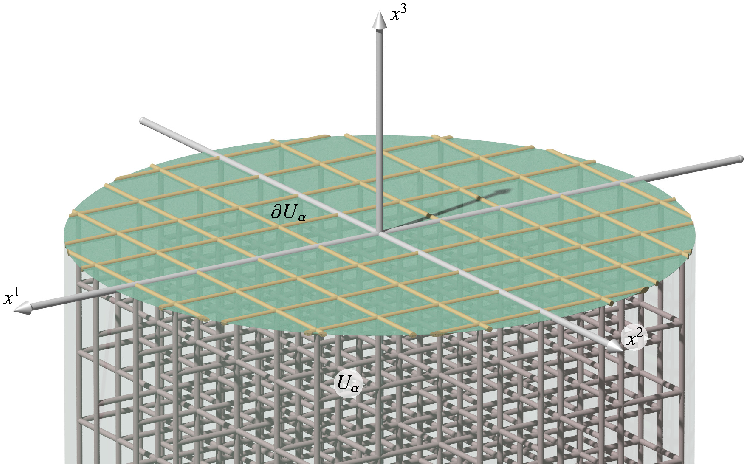
\includegraphics[width=\textwidth]{chapters/050-gauss/images/gaussrand.pdf}
\caption{Rand $\partial U_\alpha$ einer Karte $U_\alpha$ einer
dreidimensionalen Mannigfaltigkeit mit Rand für die Herleitung des
Satzes von Gauss.
\label{buch:gauss:fig:gaussrand}}
\end{figure}

Die zentrale Idee im Satz von Green war, dass sich das Integral
der Ableitung einer Funktion in Richtung senkrecht sofort auswerten
lässt.
Es blieb dann ein Integral über den Rand.
Die gleiche Argumentation funktioniert auch in drei Dimensionen.

%
% Integral und Rand
%
\subsubsection{Integral und Rand}
Sei $f\colon\mathbb{R}^2\times\mathbb{R}_{\le 0}\to \mathbb{R}$
eine Funktion mit kompaktem Träger
(Abbildung~\ref{buch:gauss:fig:gaussrand}).
Das Integral der 3-Form
\[
\omega
=
\frac{\partial f}{\partial x^3}(x^1,x^2,x^3)\,dx^1\wedge dx^2\wedge dx^3
\]
ist dann
\begin{align*}
\int_V
\frac{\partial f}{\partial x^3}(x^1,x^2,x^3)\,dx^1\wedge dx^2\wedge dx^3
&=
\int_{-\infty}^0
\int_{-\infty}^{\infty}
\int_{-\infty}^{\infty}
\frac{\partial f}{\partial x^3}(x^1,x^2,x^3)
\,dx^1
\,dx^2
\,dx^3.
\intertext{Die Integrationen dürfen vertaiuscht werden, das Integral
wird dann zu}
&=
\int_{-\infty}^{\infty}
\int_{-\infty}^{\infty}
\int_{-\infty}^0
\frac{\partial f}{\partial x^3}(x^1,x^2,x^3)
\,dx^3
\,dx^1
\,dx^2
\\
&=
\int_{-\infty}^{\infty}
\int_{-\infty}^{\infty}
\Bigl[
f(x^1,x^2,x^3)
\Bigl]_{x^3=-\infty}^{x^3=0}
\,dx^1
\,dx^2
\\
&=
\int_{-\infty}^{\infty}
\int_{-\infty}^{\infty}
f(x^1,x^2,0)
\,dx^1
\,dx^2
\\
&=
\int_{\partial V} f(x^1,x^2,0) \,dx^1\wedge dx^2.
\end{align*}
Das verbleibende Integral ist also ein Integral der Funktion $f$
über den Rand.

Eine einzelne partielle Ableitung kann natürlich keine
koordinatenunabhängige Eigenschaft sein.
In drei Dimensionen gibt es drei mögliche partielle Ableitungen.
Wie im Fall des Satzes von Green kombinieren wir daher 
drei partielle Ableitungen zur 3-Form
\begin{equation}
\omega
=
\biggl(
\frac{\partial f_{23}}{\partial x^1}
+
\frac{\partial f_{13}}{\partial x^2}
+
\frac{\partial f_{12}}{\partial x^3}
\biggr)
\,dx^1\wedge dx^2\wedge dx^3.
\label{buch:gauss:3d:eqn:divform}
\end{equation}
Jeder Summand kann integriert werden, es bleibt dann für jeden
Term ein Integral über eine 2-Form.
\begin{align}
\int_V \omega
&=
\int_{\partial V} f_{23} \,dx^2\wedge dx^3
-
\int_{\partial V} f_{13} \,dx^1\wedge dx^3
+
\int_{\partial V} f_{12} \,dx^1\wedge dx^2
\label{buch:gauss:3d:eqn:gaussvorstufe}
\end{align}
Das Vorzeichen im mittleren Term kommt von der Orientierung
der Seitenflächen.
%
% fig-oberflaeche.tex
%
% (c) 2025 Prof Dr Andreas Müller
%
\begin{figure}
\centering
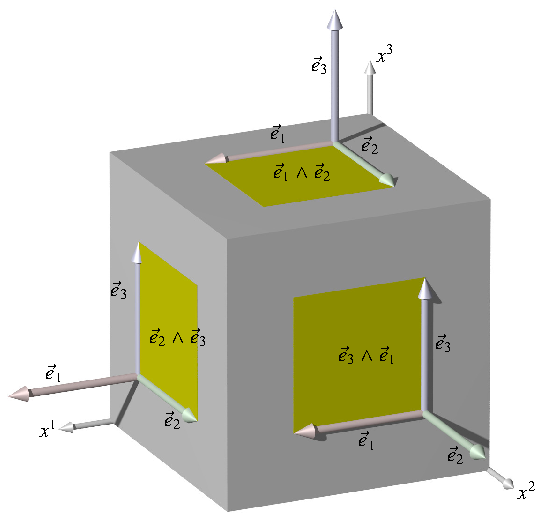
\includegraphics{chapters/050-gauss/images/oberflaeche.pdf}
\caption{Die Seitenflächen eines Koordinatenwürfels werden von den
Basis-2-Vektoren aufgespannt.
Für den Satz von Gauss müssen diese Seitenflächen untereinander kompatibel
orientiert sein.
Daher muss die von den Richtungen $\vec{e}_1$ und $\vec{e}_3$ aufgespannte
Seitenfläche die Orientierung von
$\vec{e}_3\wedge\vec{e}_1=-\vec{e_1}\wedge\vec{e_3}$
haben.
\label{buch:gauss:fig:oberflaeche}}
\end{figure}
%
In Abbildung~\ref{buch:gauss:fig:oberflaeche} sind die
2-Vektoren dargestellt, die die Seitenflächen eines achsparallelen
Würfels aufspannen.
Damit alle Seitenflächen die gleiche Orientierung verwenden, muss
die Seitenfläche senkrecht auf die $x^2$-Richtung den 2-Vektor
$\vec{e}_3\wedge\vec{e}_1=-\vec{e}_1\wedge\vec{e}_3$
verwenden.

%
% Äussere Ableitung einer 2-Form
%
\subsubsection{Äussere Ableitung einer 2-Form}
Der Ausdruck \eqref{buch:gauss:3d:eqn:divform} hat einige Ähnlichkeit
zur 2-Form, die durch äussere Ableitung einer 1-Form entsteht.
Wir definieren daher die äussere Ableitung der 2-Form
\[
\alpha
=
f_{12}(x) \,dx^1\wedge dx^2
+
f_{13}(x) \,dx^1\wedge dx^3
+
f_{23}(x) \,dx^2\wedge dx^3
\]
als
\begin{align*}
d\alpha
&=
\frac{\partial f_{12}}{\partial x^3} \,
dx^3\wedge dx^1\wedge dx^2
+
\frac{\partial f_{13}}{\partial x^2} \,
dx^2\wedge dx^1\wedge dx^3
+
\frac{\partial f_{23}}{\partial x^1} \,
dx^1\wedge dx^2\wedge dx^3.
\intertext{Durch Vertauschung der 1-Formen samt zugehörigen Vorzeichenwechseln
kann erreicht werden, dass alle Summanden Vielfache der gleichen
3-Form $dx^1\wedge dx^2\wedge dx^3$}
&=
\frac{\partial f_{12}}{\partial x^3} \,
dx^1\wedge dx^2 \wedge dx^3
-
\frac{\partial f_{13}}{\partial x^2} \,
dx^1\wedge dx^2\wedge dx^3
+
\frac{\partial f_{23}}{\partial x^1} \,
dx^1\wedge dx^2\wedge dx^3
\\
&=
\biggl(
\frac{\partial f_{23}}{\partial x^1}
-
\frac{\partial f_{13}}{\partial x^2}
+
\frac{\partial f_{12}}{\partial x^3}
\biggr)
\,dx^1\wedge dx^2\wedge dx^3.
\end{align*}
sind.

%
% Der Satz von Gauss
%
\subsubsection{Der Satz von Gauss}
Mit der äusseren Ableitung kann jetzt die
Integralbeziehung \eqref{buch:gauss:3d:eqn:gaussvorstufe}
in der Form des folgenden Satzes geschrieben werden.

\begin{satz}[Gauss]
Sie $\alpha$ eine 2-Form auf einer 3-dimensionalen Mannigfaltigkeit
$V$ mit Rand $\partial V$.
Dann gilt
\begin{equation}
\int_V d\alpha = \int_{\partial V}\alpha.
\label{buch:gauss:3d:satz:gauss:eqn}
\end{equation}
\end{satz}

Rein formal hat der Satz von Gauss die gleiche Form wie der
Satz von Stokes~\ref{buch:green:green:satz:stokes}.
Da auch der Beweis genau nah dem gleichen Muster erfolgt,
kann man vermuten, dass sich die Begriffe der $p$-Formen, der
äusseren Ableitung und des Integrals einer $p$-Form auf
beliebige Dimensionen verallgemeinern lässt.
Dies wird später in Kapitel~\ref{chapter:pformen} durchgeführt.

%
% Divergenz eines Vektorfeldes
%
\subsubsection{Divergenz eines Vektorfeldes}
In der klassischen Vektoranalysis wird die {\em Divergenz} eines Vektorfeldes
\index{Divergenz}%
$\vec{v}$ mit den Komponenten $v^i$, $i=1,\dots,3$, als
\[
\operatorname{div}\vec{v}
=
\frac{\partial v^1}{\partial x^1}
+
\frac{\partial v^2}{\partial x^2}
+
\frac{\partial v^3}{\partial x^3}
\in
\mathbb{R}.
\]
Das Integral 3-Form auf der linken Seite von
\eqref{buch:gauss:3d:satz:gauss:eqn}
im Satz von Gauss entspricht also einem Volumenintegral
der Divergenz.
Die rechte Seite von \eqref{buch:gauss:3d:satz:gauss:eqn}
ist ein Integral über eine Summe von Integranden der Form
$f_{ik}(x)\,dx^i\wedge dx^k$.
Die 2-Form $dx^i\wedge dx^k$ berechnet die Projektion eines
Parallelepipeds auf die Ebene aufgespannt von den Vektoren
$\vec{e}_i$ und $\vec{e}_k$.
Schreibt man $\vec{n}$ für die Normale eines Parallelepipeds
der Oberfläche von $V$, dann kann man den Integranden
auf der rechten Seite von \eqref{buch:gauss:3d:satz:gauss:eqn}
als das Skalarprodukt $\vec{v}\cdot d\vec{n}$ interpretieren.
In der klassischen Form wird der Satz von Gauss daher auch
in der Form
\[
\underset{V}{\int\!\!\!\int\!\!\!\int}
\operatorname{div}\vec{v}
\,dx\,dy\,dz
=
\int_{\partial V}\vec{v}\cdot d\vec{n}.
\]
geschrieben.


%
% Der Satz von Gauss
%
\section{Der verallgemeinerte Satz von Gauss
\label{buch:gauss:section:satzvongauss}}
\kopfrechts{Der verallgemeinerte Satz von Gauss}
Der Fall $n=3$ ist nicht speziell.
Die Theorie von Abschnitt~\ref{buch:gauss:section:dimension3}
kann auf beliebige $n$-dimensionale Mannigfaltigkeiten mit Rand
verallgemeinert werden.
In diesem Abschnitt ist daher $V$ eine $n$-dimensionale Mannigfaltigkeit.

% 
% n-Vektoren und n-Formen
%
\subsection{$n$-Vektoren und $n$-Formen}
Das Levi-Cività-Symbol kann verwendet werden, um den eindimensionalen
Raum der $n$-Vektoren mit dem Basisvektor
\[
\vec{e}_1\wedge\dots\wedge \vec{e}_n
=
\sum_{i_1,\dots,i_n=1}^n
\varepsilon_{i_1\dots i_n}
\,
\vec{e}_{i_1}\otimes\dots\otimes\vec{e}_{i_n}
\]
aufzuspannen.

Dual dazu ist eine $n$-Form das Produkt
\[
\omega
=
f(x)
\,
dx^1\wedge\dots\wedge dx^n.
\]
Wie im Fall $n=3$ kann man zeigen, dass das Transformationsgesetz
für eine solche $n$-Form die Multiplikation mit der Determinante
der $n\times n$-Matrix $Dy$ ist.
Dies ist die Funktionaldeterminanten einer $n$-dimensionalen
Koordinatentransformation.

%
% n-1-Vektoren und n-1-Formen
%
\subsection{$n-1$-Vektoren und $n-1$-Formen}
$n-1$-Vektoren sind Linearkombinationen
\[
\sum_{1\le i_1<\dots<i_{n-1}\le n}
a_{i_1\dots i_{n-1}}
\vec{e}_{i_1}\wedge\dots\wedge \vec{e}_{i_{n-1}}
\]
von $\wedge$-Produkt von jeweils $n-1$ Vektoren aus den Basisvektoren
$\vec{e}_1,\dots\vec{e}_n$.
Ein Basis-$n-1$-Vektor ist ein $\wedge$-Produkt von $n-1$ von den $n$
Basisvektoren.
Er stellt ein $n-1$-dimensionales Parallelepiped dar, welches senkrecht
auf der Richtung des fehlenden Vektors steht.

Im Fall $n=3$ messen 2-Formen die Projektion eines Parallelogramms
oder 2-Vektors auf die Ebene, die zu dieser 2-Form gehört.
Die Basis-2-Formen entstehen als Wedge-Produkt
\[
dx^1\wedge\dots\wedge \widehat{dx^i}\wedge\dots\wedge dx^n
\]
von $n-1$ Basis-1-Formen, wobei genau eine der 1-Formen fehlt,
nämlich die durch den Hut gekennzeichnete 1-Form $dx^i$.
Die fehlende 1-Form gehört zur Richtung senkrecht auf das
$n-1$-dimensionale Parallelepiped, das von den anderen Vektoren
aufgespannt wird.

%
% Die äussere Ableitung
%
\subsection{Die äussere Ableitung}
Für die Formulierung des Satzes von Gauss wird ausserdem die
äussere Ableitung eine $n-1$-Form benötigt.
Da der Operator der äusseren Ableitung linear ist, muss er nur
auf Basis-$n-1$-Formen definiert werden.
Wir betrachten daher die $n-1$-Form
\[
\alpha
=
a_i(x)\, dx^1\wedge\dots\wedge \widehat{dx^i}\wedge\dots\wedge dx^n.
\]
Die äussere Ableitung leitete nach der Variablen $x^i$ ab und fügt
die 1-Form $dx^i$ zum Wedge-Produkt hinzu.
Wie im Fall $n=3$ muss das Vorzeichen jeweils so angepasst werden,
dass die Orientierung der $n-1$-Form mit der Orientierung
$dx^1\wedge\dots\wedge dx^n$ kompatibel ist.
Daher muss
\begin{equation}
d\alpha
=
(-1)^{i-1}
\frac{\partial a_i(x)}{\partial x^i}
\,
dx^1\wedge\dots\wedge dx^n
\label{buch:gauss:nd:eqn:d}
\end{equation}
gesetzt werden.
Man kann dies auch wie folgt definieren.

\begin{definition}
Die {\em äussere Ableitung} der $n-1$-Form
\[
\alpha = a(x)\, dx^{i_1}\wedge\dots\wedge dx^{i_{n-1}}
\]
ist
\begin{equation}
d\alpha
=
\frac{\partial a}{\partial x^i}(x)
\,dx^i
\wedge dx^{i_1}\wedge\dots\wedge dx^{i_{n-1}}.
\label{buch:gauss:nd:eqn:dabl}
\end{equation}
\end{definition}

Da der Raum der $n$-Formen eindimensional ist, kann 
das Wedge-Produkt in \eqref{buch:gauss:nd:eqn:dabl}
immer so umgestellt werden, dass die $n$-Form
$dx^1\wedge\dots\wedge dx^n$ entsteht.
Im Falle der $n-1$-Form
\[
dx^1\wedge\dots\wedge\widehat{dx^i}\wedge\dots\wedge dx^n
\]
bedeutet dies, dass die 1-Form $dx^i$ in
\[
dx^i
\wedge
dx^1\wedge\dots\wedge\widehat{dx^i}\wedge\dots\wedge dx^n
\]
mit $i-1$ Vertauschungen an den ``richtigen'' Platz gebracht
werden kann.
Dies bringt ein Vorzeichen $(-1)^{i-1}$, welches auch in
\eqref{buch:gauss:nd:eqn:d}
wiedergefunden werden kann.

%
% Der Satz von Gauss
%
\subsection{Der Satz von Gauss
\label{buch:gauss:gauss:subsection:satzvongauss}}
\kopfrechts{Der Satz von Gauss}
Der Satz von Gauss kann jetzt für beliebige Dimension $n$ formuliert
werden.
Auf einer $n$-dimensionalen Mannigfaltigkeit ist die Integration
einer $n$-Form definiert.
Der Rand einer $n$-dimensionalen Mannigfaltigkeit ist $n-1$-dimensional,
auf dem Rand ist daher die Integration einer $n-1$-Form definiert.
Eine $n-1$-Form $\omega$ auf der Mannigfaltigkeit hat als äussere 
Ableitung eine $n$-Form $d\omega$.
Der Satz von Gauss verbindet das $n$-Form-Integral von $d\alpha$
über die ganze Mannigfaltigkeit mit dem $n-1$-Form-Integral von $\alpha$
über den Rand der Mannigfaltigkeit.

\begin{satz}[Gauss]
\index{Satz!von Gauss}%
Sei $M$ eine $n$-dimensionale Mannigfaltigkeit mit Rand $\partial M$
und $\omega$ eine $n-1$-Form auf $M$.
Dann gilt
\[
\int_M d\omega
=
\int_{\partial M} \omega.
\]
\end{satz}

%
% fig-kuh.tex
%
% (c) 2025 Prof Dr Andreas Müller
%
\begin{figure}
\centering
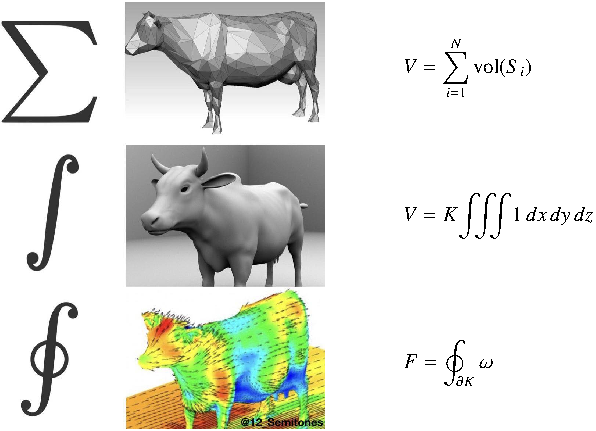
\includegraphics{chapters/050-gauss/images/kuh.pdf}
\caption{Internet-Meme, welches den Unterschied zwischen diskreter
Volumenberechnung, Volumenintegral und Flussintegral über die
Oberfläche eines Körpers illustriert.
\label{buch:gauss:fig:kuh}}
\end{figure}
%
Das Internet-Meme vom Abbildung~\ref{buch:gauss:fig:kuh} versucht,
die Idee des Integrals über den Rand einer Mannigfaltigkeit
mit Rand humoristisch zu interpretieren.
Tatsächlich ist ein solches Integral nicht nur für den Satz von Gauss
von Nutzen.
In der Elastizitätstheorie geht man davon aus, dass auf einem Element
\index{Elastizitatstheorie@Elastizitätstheorie}%
der Oberfläche, also auf einem infinitesimalen 2-Vektor, sowohl Druckkräfte
orthogonal auf das Parallelepiped wirken, als auch Scherkräfte parallel 
\index{Scherkrafte@Scherkräfte}%
zur Ebene des Parallelepipeds.
Das Integral dieser Kräfte ergibt die resultierende Kraft auf den Körper.
Die Kräfte haben auch Drehmomente zur Folge.
Falls sich der Körper nicht in Drehbewegung versetzen kann, muss
das Integral dieser Drehmomente über die ganze Oberfläche
Null ergeben.


%
% Erhaltungssätze
%
\section{Erhaltungssätze
\label{buch:gauss:section:erhaltungssatz}}
\kopfrechts{Erhaltungssätze}
Das Oberflächenintegral einer 2-Form berechnet den Fluss von Materie,
Energie oder anderen physikalischen Grössen durch die Oberfläche.
Ein Erhaltungssatz beschreibt, ob und wie der Fluss die im umschlossenen
Volumen enthaltene Menge verändert.
Der Satz von Gauss stellt den Zusammenhang her zwischen Inhalt und Fluss
über das ganze Volumen und seine Oberfläche und der, die beschreibt,
was in der unmittelbaren Umgebung jedes Punktes geschieht.
Das Resultat ist die Kontinuitätsgleichung, die in diesem Abschnitt
hergeleitet und angewendet werden soll.

%
% Kontinuitätsgleichung
%
\subsection{Kontinuitätsgleichung}
%
% fig-kont.tex
%
% (c) 2025 Prof Dr Andreas Müller
%
\begin{figure}
\centering
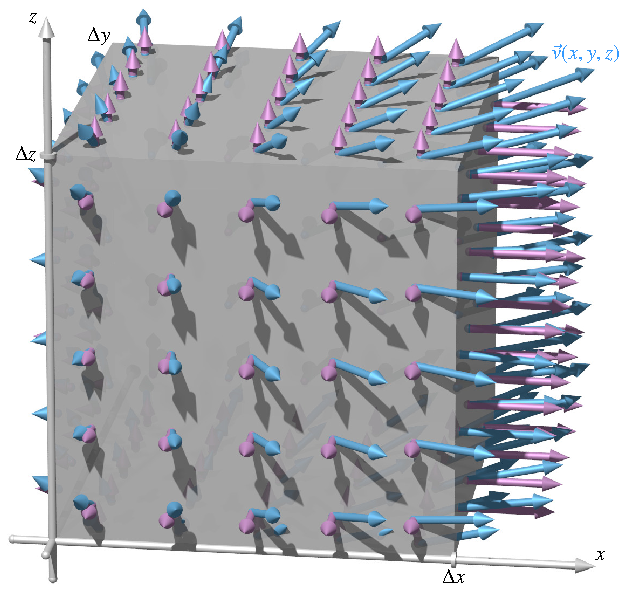
\includegraphics{chapters/050-gauss/images/kont.pdf}
\caption{Fluss des blauen Vektorfeldes durch einen Quader.
Nur die auf der Oberfläche senkrechte, violette Komponente trägt
zum Fluss bei.
\label{buch:gauss:fig:kont}}
\end{figure}
%
Wir betrachten das Vektorfeld $\vec{v}(x,y,z)$ im $\mathbb{R}^3$.
Es beschreibt die Geschwindigkeit eines Fluids der Dichte $\varrho(x,y,z)$.

Wir berechnen den Fluss des Fluids durch die Oberfläche eines Quaders
mit den Seiten $\Delta x$, $\Delta y$ und $\Delta z$.
Der Strom des Fluids ist
$\vec{\jmath}(x,y,z,t)=\varrho(x,y,z,t)\,\vec{v}(x,y,z,t)$.
Die 2-Form für den Fluss ist
\[
\omega
=
\varrho
j_x
\,dy\wedge dz
+
j_y
\,dx\wedge dz
-
j_z
\,dx\wedge dy.
\]
Der Fluss ist das Integral von $\omega$ über die Oberfläche des
Quaders.
Wir nehmen an, dass $\Delta x$, $\Delta y$ und $\Delta z$ klein
sind, so dass es gerechtfertigt ist, die Komponenten von $v$ auf
den Seitenflächen des Quaders als konstant anzusehen.
Dann ist der Fluss näherungsweise
\begin{align*}
\int_{\text{Quader}}\omega
&\approx
\Delta x\,\Delta y\,(j_z(x, y, z+\Delta z) - j_z(x, y, z))
+
\Delta x\,\Delta z\,(j_y(x, y+\Delta y, z) - j_y(x, y, z))
\\
&
\qquad
+
\Delta y\,\Delta z\,(j_x(x+\Delta x, y, z) - j_x(x, y, z))
\intertext{Gehen die Seitenlängen gegen $0$, geht auch das Integral
gegen 0.
Teilt man durch das Volumen $V=\Delta x\,\Delta y\,\Delta z$, bleibt}
\frac{1}{V}\int_{\text{Quader}} \omega
&=
\frac{j_z(x, y, z+\Delta z) - j_z(x, y, z)}{\Delta x}
+
\frac{j_y(x, y+\Delta y, z) - j_y(x, y, z)}{\Delta y}
\\
&\qquad
+
\frac{j_x(x+\Delta x, y, z) - j_x(x, y, z)}{\Delta z}
\intertext{Der Grenzwert für $\Delta x\to 0$, $\Delta y\to 0$ und
$\Delta z\to 0$ wird}
&\to
\frac{\partial j_z}{\partial z}
+
\frac{\partial j_y}{\partial y}
+
\frac{\partial j_x}{\partial x}
=
\operatorname{div}\vec{\jmath}(x,y,z).
\end{align*}
Die Divergenz misst also den Fluss durch einen infinitesimalen 
Quader.

Der Fluss beschreibt auch, mit welcher Geschwindigkeit sich die Menge
des Materials im Quader ändert.
Dies kann jedoch berechnet werden, indem die Masse zu verschiedenen
Zeiten berechnet wird.
Mit der Dichte $\varrho(x,y,z,t)$ des Fluids ist die Änderung der 
Masse gegeben durch
\begin{align*}
\Delta m
&=
\int_{\text{Quader}} \varrho(x,y,z,t+\Delta t)\,dx\,dy\,dz
-
\int_{\text{Quader}} \varrho(x,y,z,t)\,dx\,dy\,dz.
\intertext{Für einen kleinen Quader kann man wieder annehmen, dass die
Dichte im Quader im Wesentlichen konstant ist, der Masseunterschied
lässt sich daher als}
\Delta m
&\approx
(\varrho(x,y,z,t+\Delta t)
-
\varrho(x,y,z,t))
\,\Delta x\,\Delta y\,\Delta z.
\end{align*}
Die zeitliche Änderung der Dichte ist
\begin{align*}
\frac{\Delta m}{\Delta x\,\Delta y\,\Delta z\,\Delta t}
&=
\frac{\varrho(x,y,z,t+\Delta t)-\varrho(x,y,z,t)}{\Delta t}
\end{align*}
Der Grenzwert $\Delta t\to 0$ ergibt die Zeitableitung von $\varrho$
und damit die Gleichung
\begin{equation}
\frac{\partial \varrho}{\partial t}
=
\operatorname{div}\vec{\jmath}
=
\operatorname{div}(\varrho\vec{v}).
\label{buch:gauss:erhaltungssatz:eqn:kontinuitaet}
\end{equation}
Dies ist die {\em Kontinuitätsgleichung}.

%
% Anwendungen
%
\subsection{Anwendungen}
Die Kontinuitätsgleichung tritt in vielfältiger Form in den verschiedensten
Gebieten auf.

%
% Wärmeleitung
%
\subsubsection{Wärmeleitung}
Wir betrachten die Verteilung von Wärmeenergie in einem Festkörper.
Die Energiedichte $\varrho$ kann aus der orts- und zeitabhängigen
Temperatur $T(x,y,z,t)$ und der spezifischen Wärme $c$ des Materials
durch $\varrho = cT$ berechnet werden.

Der Wärmefluss in Richtung des Vektors $\vec{v}$ ist proportional
zur Temperaturdifferenz in diese Richtung:
\[
\frac{d}{ds}
T(x+s\vec{v},t)\bigg|_{s=0}
=
D_{\vec{v}} T.
\]
Die Richtungsableitung kann durch das Differential von $T$
ausgedrückt werden.
Die Koeffizienten von $dT$ sind die partiellen Ableitungen
\[
dT
=
\frac{\partial T}{\partial x}\,dx
+
\frac{\partial T}{\partial y}\,dy
+
\frac{\partial T}{\partial z}\,dz
\]
Der Proportionalitätsfaktor ist die Wärmeleitfähigkeit $\kappa$.
Damit wird der Wärmestrom:
\[
j_x\,dx
+
j_y\,dy
+
j_z\,dz
=
\kappa
dT
\qquad\text{oder}\qquad
\vec{\jmath}
=
\kappa
\operatorname{grad} T
\]
in vektorieller Schreibweise.
Die Erhaltung der Energie wird durch die Kontinuitätsgleichung
für die Energiedichte $\varrho$ und den Stromvektor $\vec{\jmath}$
ausgedrückt.
Durch die Temperatur ausgedrückt besagt sie
\[
\frac{\partial }{\partial t}
(cT)
=
\operatorname{div}(\kappa\operatorname{grad}T).
\]

In einem homogenen Medium darf man annehmen, dass $c$ und $\kappa$ konstant
sind.
Die Kontinuitätsgleichung wird damit zu
\begin{align*}
c\frac{\partial T}{\partial t}
&=
\kappa
\operatorname{div}\operatorname{grad}T
\\
&=
c
\biggl(
\frac{\partial}{\partial x}
\frac{\partial T}{\partial x}
+
\frac{\partial}{\partial y}
\frac{\partial T}{\partial y}
+
\frac{\partial}{\partial z}
\frac{\partial T}{\partial z}
\biggr)
\\
&=
\kappa
\biggl(
\frac{\partial^2 T}{\partial x^2}
+
\frac{\partial^2 T}{\partial y^2}
+
\frac{\partial^2 T}{\partial z^2}
\biggr)
=
\kappa \Delta T
\end{align*}
mit dem Laplace-Operator $\Delta$.

%
% Elektrische Ladung
%
\subsubsection{Elektrische Ladung}
Die elektrische Ladung ist erhalten.
Die elektrische Stromdichte $\vec{\jmath}$ ist der Vektor, der die Ladung
angibt, die in einer Zeiteinheit durch eine Flächeneinheit quer zur
Stromrichtung angibt.
Für die Ladungsdichte $\varrho$ und die Stromdichte $\vec{\jmath}$
muss daher die Kontinuitätsgleichung
\[
\frac{\partial\varrho}{\partial t}
=
\operatorname{div} \vec{\jmath}
\]
gelten.

%
% Erhaltungssätze für Vierervektoren
%
\subsubsection{Erhaltungssätze für Vierervektoren}
In der speziellen Relativitätstheorie wird gelehrt, dass Raum- und
Zeitkoordinaten nicht separat behandelt werden sollten, sondern als
Komponenten eines Raum-Zeit-Kontinuums.
Eine Lorentz-Transformation kann Orts- und Zeitkoordinaten  ``vermischen''
was zu den Phänomen der Zeitdilatation und der Raumkontraktion führt.
Es beutet, dass zu vektoriellen Grössen, mit denen man in der newtonschen
Mechanik rechnet, jeweils auch eine Zeit-Komponenten gefunden werden
muss.
Zusammen bilden diese Komponenten einen Vierervektor, der die gleichen
Transformationsregeln befolgt, wie Ort und Zeit.
Das Skalarprodukt solcher Vierervektoren mit sich selbst bleibt
bei Lorentz-Transformationen erhalten.
Das Skalarprodukt eines Viervektors $x^k$ in der speziellen
Relativitätstheorie ist
\[
(x^0)^2
-
(x^1)^2
-
(x^2)^2
-
(x^3)^2,
\]
welches auch durch den metrischen Tensor
\[
(g_{ik})
=
\begin{pmatrix}
1&0&0&0\\
0&-1&0&0\\
0&0&-1&0\\
0&0&0&-1
\end{pmatrix}
\]
beschrieben werden kann.

Für den elektrischen Strom mit den Komponenten $j_1,j_2,j_3$ ist die
zugehörige Zeitkomponenten die Ladungsdichte, wir sind also gezwungen
$j_0=\varrho$ zu schreiben.
Die Kontinuitätsgleichung
\begin{align*}
\frac{\partial\varrho}{\partial t}
&=
\frac{\partial j_1}{\partial x^1}
+
\frac{\partial j_2}{\partial x^2}
+
\frac{\partial j_3}{\partial x^3}
\intertext{bekommt dann die Form}
\frac{\partial j_0}{\partial x^0}
&-
\frac{\partial j_1}{\partial x^1}
-
\frac{\partial j_2}{\partial x^2}
-
\frac{\partial j_3}{\partial x^3}
=
0.
\end{align*}
Dies kann etwas kompakter auch als
\[
\sum_{i,k=0}^3
g^{ik}\frac{\partial}{\partial x^k}j_i
=
0
\]
geschrieben werden kann.
Dies deutet an, dass es einen Differentialoperator, die Viererdivergenz,
gibt, der die Ladungserhaltung beschreiben kann.
Die genaue Definition wird in Kapitel~\ref{chapter:hodge} mit Hilfe des
Hodge-Operators gegeben.




